\documentclass[12pt]{amsart}
\usepackage{amssymb,amsmath,amsthm,latexsym}
\usepackage{mathrsfs}
\usepackage{a4wide}
%\usepackage{eucal}
\usepackage[usenames,dvipsnames]{color}
%\usepackage{stackengine}
\usepackage[utf8]{inputenc}
\usepackage[T1]{fontenc}
\usepackage{dsfont}
\usepackage{tikz}
\usepackage{float}
\usepackage[mathscr]{euscript}
\usepackage{mathtools}
\usepackage{hyperref}

\newtheorem{theorem}{Theorem}[section]
\newtheorem*{maint}{{\textbf{Theorem}}}
\newtheorem*{maintb}{{\textbf{Theorem A}}}
\newtheorem*{maintbb}{{\textbf{Theorem B}}}
\newtheorem*{maintbprime}{{\textbf{Theorem A${}^\prime$}}}
\newtheorem{lemma}[theorem]{Lemma}
\newtheorem{corollary}[theorem]{Corollary}
\newtheorem{proposition}[theorem]{Proposition}
\theoremstyle{remark}

\newtheorem{remark}[theorem]{Remark}
\newtheorem*{remark*}{Remark}
\theoremstyle{definition}
\newtheorem{definition}{Definition}
\newtheorem{problem}{Problem}
\newtheorem{example}[theorem]{Example}
\numberwithin{equation}{section}
\makeatother
\author{Micha\l \ Gnacik}
\newcommand{\eten}{\widecheck{\otimes}\,}

\newcommand{\vertiii}[1]{{\left\vert\kern-0.25ex\left\vert\kern-0.25ex\left\vert #1 
		\right\vert\kern-0.25ex\right\vert\kern-0.25ex\right\vert}}

\newcounter{smallromans}
\renewcommand{\thesmallromans}{\roman{smallromans}}
\newenvironment{romanenumerate}
{\begin{list}{{\normalfont\textrm{(\roman{smallromans})}}}%
		{\usecounter{smallromans}\setlength{\itemindent}{0cm}%
			\setlength{\leftmargin}{5.5ex}\setlength{\labelwidth}{5.5ex}%
			\setlength{\topsep}{.5ex}\setlength{\partopsep}{.5ex}%
			\setlength{\itemsep}{0.1ex}}}%
	{\end{list}}

\newcommand{\romanref}[1]{{\normalfont\textrm{(\ref{#1})}}}

\newcounter{smallromansdash}
\renewcommand{\thesmallromansdash}{\roman{smallromansdash}}
\newenvironment{romandashenumerate}
{\begin{list}{{\normalfont\textrm{(\roman{smallromansdash}$'$)}}}%
		{\usecounter{smallromansdash}\setlength{\itemindent}{0cm}%
			\setlength{\leftmargin}{5.5ex}\setlength{\labelwidth}{5.5ex}%
			\setlength{\topsep}{.5ex}\setlength{\partopsep}{.5ex}%
			\setlength{\itemsep}{0.1ex}}}%
	{\end{list}}

\newcounter{bigromans} \renewcommand{\thebigromans}{\Roman{bigromans}}
\newenvironment{capromanenumerate}
{\begin{list}{{\normalfont\textrm{(\Roman{bigromans})}}}%
		{\usecounter{bigromans}\setlength{\itemindent}{0cm}%
			\setlength{\leftmargin}{5.5ex}\setlength{\labelwidth}{6ex}%
			\setlength{\topsep}{.5ex}\setlength{\partopsep}{.5ex}%
			\setlength{\itemsep}{0.1ex}}}%
	{\end{list}}

\title[Intro to NN]{Notes: Introduction to Artificial Neural Networks
}


\begin{document}
\maketitle

In this set of notes we provide all the elements that allow the reader to code all described neural networks from scratch. We are not providing the details regarding the convergence of certain algorithms. As the main reference on various neural networks we refer the reader to \cite{bishop:2006:PRML}.

\section{Feedforward Neural Networks}
Let $n, m \in \mathbb{N}$ and let $x= (x_1, \ldots, x_n), y=(y_1, \ldots, y_m) \in \mathbb{R}^m$ be the input vector (one element of a training data set) and the desired output vector, respectively. Here $n$ represents the number of features (predictors) and the $y$ is the response (or the target). We aim to construct a network so that given the input $x$ the output $\widehat{y}$ is obtained 
so that $\| y - \widehat{y}\|^2$ is as small as possible.

\noindent  
We consider a network or directed acyclic graph $G = (V, E)$ ($V$ is a set of vertices or nodes and $E$ is a set of all edges (between nodes)) with the following structure of layers (organised disjoint blocks of graph vertices/nodes/neurons), see also Figure \ref{fig: nn}.  
\begin{figure}[h!]
	\centering
	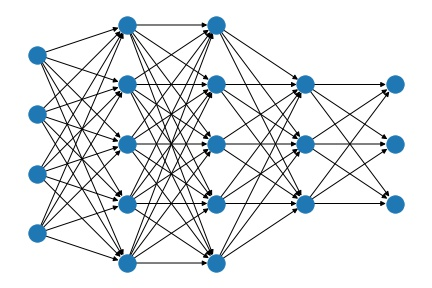
\includegraphics[scale=0.5]{nn.jpg}
	\caption{A feedforward neural network with input of size 3, three hidden layers and output of size 2.}
	\label{fig: nn}
\end{figure}
 
\begin{enumerate}
	\item \textbf{Input layer}; each node of this layer corresponds to $x_i$ for $1 \leq i \leq n$, none of the nodes within this layer are connected by edges. 
	\item \textbf{Hidden layers}; first fix the number of hidden layers $n_h \geq 0$. Assume that $k$-th hidden layer has $r_k \in \mathbb{N}$ nodes (setting $r_0 = n$ so the input layer has $n$ nodes and $r_{n_h +1} = m$ so that the output layer has $m$ nodes). Each of the nodes from the input layer is connected (forward only) with the first hidden layer with specified weights, none of the nodes within a single hidden layer are connected by edges, each of the node of the hidden layer is connected to each of the node of the next layer (forward connection only), in particular, the last hidden layer is connected forward with the output layer. 
	\item \textbf{Output layer}; the number of the nodes of this layer correspond to the number of the coordinates of $y$ vector. As mentioned earlier, each of the node is connected with each of the node of the previous (last hidden) layer, but the direction is forward, that is, one can travel from the previous layer to output layer but not vice-versa.   
\end{enumerate} 

There are $n_h+1$ matrices $W_{k}= [w_{ij}^{(k)}]$ whose entries correspond to the weights between the nodes of $k-1$ and $k$ layer, and $n_h+1$ vectors $B_k= (b_1^{(k)}, \ldots, b_{r_k}^{(k)})$ for $k \in \{1, \ldots, n_h+1\}$ that contain the bias (constant value that shifts the activation from the origin) for the nodes. 

\begin{remark}
A feedforward neural network with no hidden layers is also known a \emph{perceptron}. One may think about the feedforward neural network as a composition of perceptrons, and refer to it as the multi-layer perceptron (MLP).  
\end{remark}

We describe how the network output $\widehat{y} \in \mathbb{R}^m$ is obtained in the next section. 
\subsection{Feeding forward}

Assume that $i$-th hidden layer is equipped with an activation function $g_i$ for $i \in \{1, \ldots, n_h\}$ and the output layer is equipped with the activation function $g_{n_h+1}:=g_{\mathsf{out}}$. Here we list a few examples of differentiable activation functions: 
\begin{example}\enskip 
	\begin{enumerate}
		\item identity: $I(x)=x$ with range $\mathbb{R}$.
		\item sigmoid function: $\sigma(x) = \frac{1}{1+e^{-x}}$ has range $(0, 1]$.
		\item hyperbolic tangent:  $g(x) = \tanh{x} = \frac{e^x + e^{-x}}{e^{x}-e^{-x}}$ has range $(-1, 1)$.
		\item SoftPlus: $f(x) = \ln(1+e^x)$ has range $(0, \infty)$.
	\end{enumerate}
Note that all but first one, are non-linear. Only non-linear activation functions enable networks to compute non-trivial problems using a small number of neurons. 
\end{example}



First note that the size of each $W_{k}$ matrix is $r_{k-1} \times r_{k}$ for $k \in \{1, \ldots, n_h+1\}$. We will use the following notation, $W_k[:, j]$ is the $j$-th column of $W_{k}$ matrix. 

Obtaining $\widehat{y}$ is achieved by the following iterative process:
\noindent for brevity set $a^{(0)} := x$ so that $a^{(0)} = (a^{(0)}_1, \ldots, a^{(0)}_{n})$. At each neuron (node) of the first hidden layer we arrive at the following quantities:
\begin{align*}
z_k^{(1)} :=& \left< a^{(0)}, W_{1}[:, k]\right> + b_k^{(1)} = \sum_{j=1}^{r_0} a_{j}^{(0)}w_{jk}^{(1)} +  b_k^{(1)},\\
a_k^{(1)} :=& g_{1}(z_k^{(1)}),
\end{align*}
the latter is referred to as the output of that node.
Also denote 
$z^{(1)} = (z_1^{(1)}, z_2^{(1)},\ldots, z_{r_1}^{(1)})$ and $a^{(1)} = (a_1^{(1)}, a_2^{(1)},\ldots, a_{r_1}^{(1)})$.
Alternatively, one may obtain $z^{(1)}$ via matrix operations
$$z^{(1)} = {(a^{(0)})}^T W_1 + B_1,$$
where $T$ denotes the transpose. 

\noindent 
We iterate so that at $l$-th layer ($l \in \{2, \ldots, n_h+1\}$) we obtain
\begin{align*}
z_k^{(l)} :=& \left< a^{(l-1)}, W_{l}[:, k]\right> + b_k^{(l)} = \sum_{j=1}^{r_{l-1}} a_{j}^{(l-1)}w_{jk}^{(l)} +  b_k^{(l)},\\
a_k^{(l)} :=& g_{l}(z_k^{(l)})
\end{align*}
and similarly, denoting 
$z^{(l)} = (z_1^{(l)}, z_2^{(l)},\ldots, z_{r_l}^{(l)})$, $a^{(l)} = (a_1^{(l)}, a_2^{(l)},\ldots, a_{r_l}^{(l)})$.
Alternatively, one may find $z^{(l)}$ via matrix operations
$$z^{(l)} = \left(a^{(l-1)}\right)^TW_l + B_l.$$
\noindent 
Finally we obtain the output from our network as 
$$ \widehat{y}_k = a_{k}^{(n_h+1)} \ \ (k = 1, \ldots, m).$$
\begin{remark} \enskip 
	\begin{itemize} 
\item When initilising the network (before we train it with data) we set up the network with random weights (e.g. drawn from uniform distribution on $[-1, 1]$) and biases and adjust them later via, e.g., gradient descent so that prediction error is minimal (here one needs to run cross validation to avoid overfitting).
\item Note that the range of activation function $g_{n_h+1}$ needs to be consistent with the values of $y$. 
%\item If activation functions are linear the problem can be reduced to the two-layer input-output network with non-hidden layers. 
\end{itemize}
\end{remark}
\subsection{Backpropagation}

Define the cost function for a single iteration $K$-th iteration
$$ C_K = \sum_{i=1}^m (\widehat{y}_i - y_i)^2.$$
For brevity, in this section, we drop the subscript $K$ so write $C \equiv C_K$.
We wish to minimise $C$ treated as a function of weights and biases. 
In order to that one may employ, e.g., gradient descent method, for that we would require to find 
$\frac{\partial C}{ \partial w_{ij}^{(k)} }$ and $\frac{\partial C}{ \partial b_{i}^{(k)} }$ for each $i \in \{1, \ldots, r_{k-1}\}$, $j \in \{1, \ldots, r_k\}$ and $k \in \{1, \ldots, n_h+1\}$.
The process of finding the above derivatives is referred to as backpropagation, as it is easy to find the derivatives with respect to weights and biases in the last layer, and then consider the ones from the previous layer and so on.  

We use the chain rule to obtain 
\begin{align*}
\frac{\partial C}{ \partial w_{ij}^{(n_h+1)}} = \frac{\partial C}{\partial z_j^{(n_h+1)}} \frac{\partial z_j^{(n_h+1)}}{ \partial w_{ij}^{(n_h+1)}}.
\end{align*}
Note that since $C$ is a multi-variable function, one would expect more terms in the chain rule, however these vanish as
$$\frac{\partial z_l^{(n_h+1)}}{ \partial w_{ij}^{(n_h+1)}} = \begin{cases} a_i^{(n_h)} & \mbox{ if } l=j \\ 0 & \mbox{ if } l \neq j\end{cases}.$$
Let us denote 
$$ \delta_j^{(k)}:= \frac{\partial C}{\partial z_j^{(k)}}.$$
We find that 
$$  \delta_j^{(n_h+1)}= 2(\widehat{y}_j - y_j)g^{\prime}_{\mathsf{out}}(z_j^{(n_h+1)}).$$
Hence, 
$$\frac{\partial C}{ \partial w_{ij}^{(n_h+1)}} = 2a_i^{(n_h)}(\widehat{y}_j - y_j)g^{\prime}_{\mathsf{out}}(z_j^{(n_h+1)}).
$$
For all $k \in \{1, \ldots, n_h\}$ we obtain
\begin{align*}
\frac{\partial C}{ \partial w_{ij}^{(k)}} =& \frac{\partial C}{\partial z_j^{(k)}} \frac{\partial z_j^{(k)}}{ \partial w_{ij}^{(k)}}\\
=& \delta_j^{(k)} \frac{\partial z_j^{(k)}}{ \partial w_{ij}^{(k)}}.
\end{align*}
We have
$$
\frac{\partial z_j^{(k)}}{ \partial w_{ij}^{(k)}} = a_i^{(k-1)}$$
For $\delta_j^{(k)}$ we apply the chain rule, thus
\begin{align*}
\delta_j^{(k)} =& \sum_{l=1}^{r_{k+1}} \frac{\partial C}{\partial z_l^{(k+1)}} \frac{\partial z_l^{(k+1)}}{\partial z_{j}^{(k)}},\\
=& \sum_{l=1}^{r_{k+1}}\delta_l^{(k+1)} \frac{\partial z_l^{(k+1)}} {\partial z_{j}^{(k)}}
\end{align*}
and
\begin{align*}
\frac{\partial z_l^{(k+1)}} {\partial z_{j}^{(k)}}
=& g_k^{\prime}(z_j^{(k)})w_{jl}^{(k+1)}.
\end{align*}
Hence, for all $k \in \{1, \ldots, n_h\}$ we have
\begin{align*}
\frac{\partial C}{ \partial w_{ij}^{(k)}} =&g_k^{\prime}(z_j^{(k)}) a_i^{(k-1)} \sum_{l=1}^{r_{k+1}}\delta_l^{(k+1)} w_{jl}^{(k+1)}\\
\frac{\partial C}{ \partial w_{ij}^{(n_h+1)}} =& \underbrace{2(\widehat{y}_j - y_j)g^{\prime}_{\mathsf{out}}(z_j^{(n_h+1)})}_{\delta_j^{(n_h+1)}}a_i^{(n_h)}.
\end{align*}
Similarly, taking into account that 
$$\frac{\partial z_j^{(k)}}{ \partial b_{i}^{(k)}}=1$$
we obtain 
\begin{align*}
\frac{\partial C}{ \partial b_{i}^{(k)}} =&g_k^{\prime}(z_j^{(k)})  \sum_{l=1}^{r_{k+1}}\delta_l^{(k+1)} w_{jl}^{(k+1)},\\
\frac{\partial C}{ \partial b_{ij}^{(n_h+1)}} =& \underbrace{2(\widehat{y}_j - y_j)g^{\prime}_{\mathsf{out}}(z_j^{(n_h+1)})}_{\delta_j^{(n_h+1)}}.
\end{align*}
for all $k \in \{1, \ldots, n_h\}$.
\subsection{Training the network}
\subsubsection{Training via gradient descent}
Given a training data set $(X, Y)$, where $X = (X_1, \ldots, X_N)$, 
$Y = (Y_1, \ldots, Y_N)$ and each $X_k \in \mathbb{R}^n$, $Y_k \in \mathbb{R}^m$ for all $k$.
Let us denote the output of our network given input $X_k$ to be $\widehat{y}_{k} \in \mathbb{R}^m$. Then in order to minimise
$$C(N) = \frac{1}{N} \sum_{i=1}^N \| \widehat{y}_i - Y_i\|^2 = \frac{1}{N} \sum_{i=1}^N C_i,$$
where $\| \cdot \|$ is a Euclidean norm in $\mathbb{R}^m$, we perform gradient descent (GD) and so use the results from backpropagation section, so that each we update the weights and biases as follows
\begin{align*} 
w_{ij}^{(k), \star} =& w_{ij}^{(k)} - \frac{\alpha}{N} \sum_{l=1}^N \frac{\partial C_l}{ \partial w_{ij}^{(k)}},\\
b_{i}^{(k), \star} =& b_{i}^{(k)} - \frac{\alpha}{N} \sum_{l=1}^N \frac{\partial C_l}{ \partial b_{i}^{(k)}},
\end{align*}
where $\alpha>0$ is so-called learning rate, and  $w_{ij}^{(k), \star}$, $b_{i}^{(k), \star}$,  represent the new weights and biases that we should consider in our neural network.  

We can iterate this process to get to the minimum as close as possible. We refer to each iteration of the above process as an epoch. To be more precise a number of epochs describes how man times the algorithm has gone through the entire training data set (full-batch)

\subsubsection{Training via stochastic gradient descent}
In stochastic gradient descent (SGD), rather than the gradient of the full-batch we use a gradient of a single (or a mini-batch of) the training data set and proceed as follows:

\begin{enumerate}
	\item randomly shuffle your training data set
	\item for $l$ in $\{1, \ldots, N\}$ update the weights and biases as follows:
	\begin{align*} 
	w_{ij}^{(k), \star} =& w_{ij}^{(k)} - \alpha \frac{\partial C_l}{ \partial w_{ij}^{(k)}},\\
	b_{i}^{(k), \star} =& b_{i}^{(k)} - \alpha \frac{\partial C_l}{ \partial b_{i}^{(k)}}.
	\end{align*}
\end{enumerate} 
An epoch is completed when you finish all $N$ iterations. A mini-batch version of SGD proceeds as follows
\begin{enumerate}
	\item randomly shuffle your training data set.
	\item Divide your data set into mini-batches $B_l$ of size $K$ (assume that $K|N$) then for $l$ in $\{1, \ldots, \tfrac{N}{K}\}$ update the weights and biases as follows:
	\begin{align*} 
	w_{ij}^{(k), \star} =& w_{ij}^{(k)} - \frac{\alpha}{|B_l|} \sum_{r \in B_l}  \frac{\partial C_r}{ \partial w_{ij}^{(k)}},\\
	b_{i}^{(k), \star} =& b_{i}^{(k)} -  \frac{\alpha}{|B_l|} \sum_{r \in B_l}   \frac{\partial C_r}{ \partial b_{i}^{(k)}}.
	\end{align*}
\end{enumerate} 
An epoch is completed when you finish all $\frac{N}{K}$ iterations. 

SGD often converges much faster than GD however the cost function may not be minimised as well as in the GD. In modern ML due to faster computation, SGD is a preferred method. 

\bibliography{Refs}{}
\bibliographystyle{unsrt}



\end{document}
